\section{Back-End Server}
The Back-End server instantiates different versions of itself based on command line arguments.
Each instance of a Back-End server is be responsible for listening for a specific type of data,
APRS data, telemetry data and video data.

\begin{figure}[!ht]
  \centering
  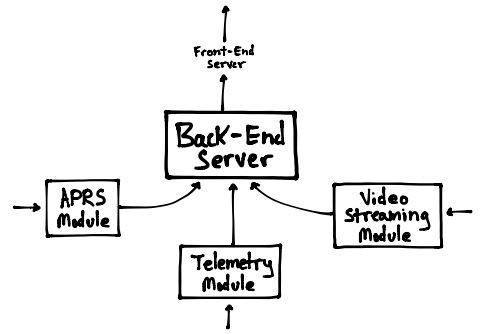
\includegraphics[scale=.8]{imgs/back-end-server.jpg}
  \caption{Back-End Server}
\end{figure}

\subsection{APRS Module}
The APRS module catches raw APRS packets sent by the Recovery Crews and sending on to the Front-End server.

\begin{figure}[!ht]
  \centering
  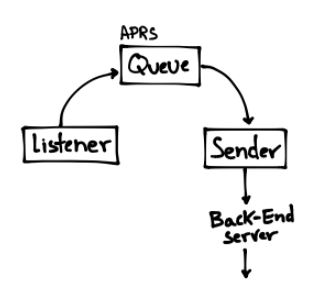
\includegraphics[scale=.8]{imgs/aprs-detailed.jpg}
  \caption{APRS module}
\end{figure}

\newpage

\subsection{Telemetry Module}
The Telemetry module catches raw telemetry data from the rocket and sending to the Front-End server.

\begin{figure}[!ht]
  \centering
  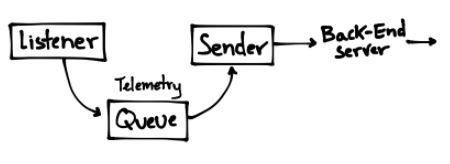
\includegraphics[scale=.8]{imgs/telemetry-detailed.jpg}
  \caption{Telemetry Module}
\end{figure}

\subsection{Video Streaming Module}
The video module catches the live video streams and sending them to the Front-End server.

\begin{figure}[!ht]
  \centering
  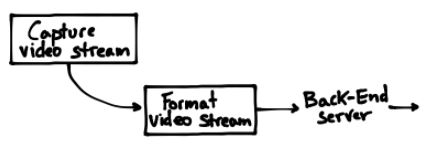
\includegraphics[scale=.8]{imgs/video-detailed.jpg}
  \caption{Telemetry Module}
\end{figure}

